%\documentclass[12pt,a4paper,twocolumn]{report}
\documentclass[10pt]{IEEEtran}
%\usepackage[top=1in, bottom=1in, left=1in, right=1in]{geometry}
\usepackage[utf8]{inputenc}
\usepackage{amsmath}
\usepackage{amsfonts}
\usepackage{amssymb}
\usepackage{graphicx}
\usepackage{mdframed}
\usepackage{multicol}

\title{ECE 520 Final Project}
\author{Christopher Johnson, Joshua Stevens}
\date{April 09, 2014}

\mdfsetup{%
	linewidth = 1pt,
	topline = true,
	bottomline = true,
	leftline = true,
	rightline = true}
	
\begin{document}

\twocolumn[{\centering
\textbf{\Large Histogram Equalizer\\}
\large \textbf{ECE 520 Final Project\\}
	Christopher Johnson, Joshua Stevens
	\normalsize
	\\[3em]

\begin{mdframed}
\textbf{Project Responsibilities:}\\
csjohns3. Christopher Johnson:\\
${}$\hspace{5em}Input Pipeline, Testbench, Top, Report \vspace*{.5em}\\
jasteve4. Joshua Stevens:\\
${}$\hspace{5em}Output Pipeline/CDF, Testbench, Top, Report\\
\end{mdframed}

%%%%%%%%%%%%%%%%%%%%%%%%%%   3 columns
\begin{multicols}{3}
	\begin{mdframed}
		\textbf{Delay (ns to run ex)} \\
		Clock period: 4.1 ns \\
		Cycles: 307466\\
	\end{mdframed}

	\begin{mdframed}
		\textbf{Area: ($\mathbf{um^{2}}$)}\\ \\
		Logic: 11928.30198 \\\\
		Memory: N/A\\
	\end{mdframed}
		
	\begin{mdframed}
		\textbf{(delay.area)(ns-1.um-2):} \\\\66.497E-12\\\\
	\end{mdframed}

\end{multicols}
%%%%%%%%%%%%%%%%%%%%%%%%%%   END 3 columns

%%%%%%%%%%%%%%%%%%%%%%%%%%   2 columns
\begin{multicols}{2}
	\begin{mdframed}
		\textbf{Delay (TA)}\\\
		Clock period: \\
		cycles: \\
	\end{mdframed}
	
	\begin{mdframed}
		\textbf{1/(delay.area) (TA)}\\
		\\
		\\
	\end{mdframed}
\end{multicols}

\emph{NOTE: The statistic above (with exception to the "TA" fields) are run using "input\_small\_hex.txt"}\\[1em]
}]
%%%%%%%%%%%%%%%%%%%%%%%%%%  END 2 columns

\textbf{\emph{Abstract} - This paper describes a hardware design responsible for improving the contrast of individual frames of a video capture device. The algorithm is based on a histogram equalizer and the hardware is heavily pipelined in order to allow a low clock speed and the ability to quickly process individual images. Using Synopsys Design Vision and Mentor Graphics ModelSim, we prove that with this chip, it is possible to process video at 793 fps with an area of 11929.3 $\mathbf{\boldsymbol\mu m^{2}}$.}
 

\section{Introduction}

When using a video capturing device, it can be quite common to achieve footage with poor pixel contrast. This is something that can be solved relatively easily using a software histogram equalizer, however; this software is generally quite slower than the image capture hardware of the camera thus creating a bottleneck. To alleviate this bottleneck, we have created a hardware histogram equalizer. Our design is heavily pipelined allowing the clock speed to be quite low and enabling multiple images to be processed at a time. The result is a hardware module that can process video at 793 fps with an area of 11929.3 $m^{2}$. This is significant because this is much smaller and faster than a comparative software/hardware combination while performing the same function.
 

\section{Micro-Architecture}

\begin{figure}[htb!]
	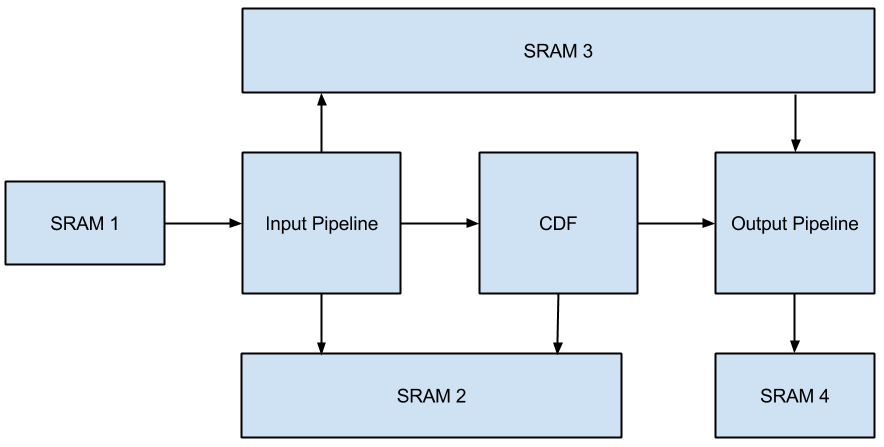
\includegraphics[width=90mm]{System_Overview.png}
	\caption{System Overview}
\end{figure}

Our overall system is divided into two major stages ("Input Pipeline/CDF Pipeline" and "Output Pipeline") that are individually pipelined and interfaced through a "Controller" module. These two stages are pipelined such that the "Input Pipeline/CDF Pipeline" module runs in approximately the same amount of time as "Output Pipeline." This allows both modules to run images simultaneously with a minimum number of unused clock cycles.

\subsection*{Input Pipeline}
This module is responsible for reading pixel values from memory and storing how many times each pixel value occurs to SRAM 2. In order to improve efficiency of this process, a five stage pipeline is used. This allows memory operations to happen in separate cycles from the accumulation stages. This is crucial since it takes 2ns to read or write to the SRAM. In order to keep this pipeline running as quickly as possible, three data bypasses were introduced for coping with the 2ns memory read/write. Finally, this module is responsible for copying the original picture from SRAM 1 to SRAM 3 so "Output Pipeline" will have the image for reference.

\subsection*{CDF Pipeline}
The sole purpose of this module is to calculate the CDF across all pixel values accumulated in the "Input Pipeline." The results are then loaded into SRAM 2. This pipeline takes the least amount of time to complete, however; it cannot run until "Input Pipeline" is complete and "Output Pipeline" cannot run until the CDF is fully calculated. For this reason, we decided to combine the "CDF Pipeline" module with the "Input Pipeline" in our overall system.

\subsection*{Output Pipeline}
"Output Pipeline" is the most process intensive module. This module requires a multiplier, a divider, and an adder to operate. In order to optimize these calculations, we chose to use pipelined binary shift multipliers and dividers. We found this to be a very effective method for calculations while providing us a lot of control over the number of pipeline stages we used. The ability to adjust the number of pipeline stages was especially helpful in making sure the "Input/CDF Pipeline" and "Output Pipeline" ran for approximately the same number of cycles. In addition to allowing us to adjust the pipeline stages, creating our own dividers and multipliers allowed us to limit the number of bits required for the quotient to meet our specific application. Adjusting these bit helped to reduce both timing and area. Finally, we chose to use the Synopsys DesignWare adder as opposed to using the '+' operator. After adding the DesignWare module, our maximum clock speed changed from approximately 10 ns to our current 4.1 ns.
 

\subsection*{Controller}
"Controller" handles the signal necessary to start and stop each pipeline as well as informing our chip where to store data in SRAM 2. By controlling where data in SRAM 2 is stored, this modules alone provides the capability of running two images through our pipeline simultaneously. To make this possible, "Controller" toggles the upper most address bit of each read and write to the SRAM 2. In doing this, our system is able to store one image in the lower half of SRAM 2 and one in the upper half of SRAM 2. Since "Input Pipeline" and "Output Pipeline" are always running 2 different images, they are always operating in opposite halves of SRAM 2.

\section{Verification}
To verify this module we used a combination of Synopsys Design Vision and Mentor Graphics Modelsim. Synopsys Design Vision was used to determine our clock speed, and to find synthesis issues in our hardware design. Modelsim was used to verify proper operation of our module. When testing for calculation accuracy in Modelsim, we used numerous test vectors that were generated by proven working C code. Through Synopsys, we were able to adjust clock speed of our verified design and note how this effected the area, thus allowing us to optimize the equation $1/(delayxarea)$.

\section{Results}
Our design ran optimally with a clock speed of 4.1 ns and an area of 11,929.3 um. This setup is capable of processing video at approximately 793 fps. 

\section{Conclusion}
Pipelining partnered with shift dividers and multipliers was very effective in creating fast and space efficient histogram equalizer. For further improvements it would be possible to design our own adder module specific to this application but this would only produce a small increase in performance.

\end{document}

